\iffalse
\documentclass[journal,12pt,twocolumn]{IEEEtran}

% Packages
\usepackage{cite}
\usepackage{amsmath,amssymb,amsfonts,amsthm}
\usepackage{graphicx}
\usepackage{textcomp}
\usepackage{xcolor}
\usepackage{txfonts}
\usepackage{listings}
\usepackage{enumitem}
\usepackage{mathtools}
\usepackage{float}
\usepackage{gensymb}
\usepackage{comment}
\usepackage{hyperref}
\usepackage{tkz-euclide}
\usepackage{gvv}
\usepackage[latin1]{inputenc}
\usepackage{color}
\usepackage{array}
\usepackage{longtable}
\usepackage{calc}
\usepackage{multirow}
\usepackage{hhline}
\usepackage{ifthen}
\usepackage{lscape}
\usepackage{subcaption}
\usepackage{tikz}
\usepackage{circuitikz}
\usepackage{wrapfig}
\usepackage{lipsum}
\usepackage[export]{adjustbox}
\usepackage{inputenc}

% Custom commands and macros
\newtheorem{theorem}{Theorem}[section]
\newtheorem{problem}{Problem}
\newtheorem{proposition}{Proposition}[section]
\newtheorem{lemma}{Lemma}[section]
\newtheorem{corollary}[theorem]{Corollary}
\newtheorem{example}{Example}[section]
\newtheorem{definition}[problem]{Definition}
\newtheorem{rem}{Remark}
\newcommand{\BEQA}{\begin{eqnarray}}
\newcommand{\EEQA}{\end{eqnarray}}
\newcommand{\define}{\stackrel{\triangle}{=}}
\renewcommand{\thefigure}{\theenumi}
\renewcommand{\thetable}{\theenumi}



\begin{document}

\title{GATE 2023 EC 49}
\author{EE23BTECH11045 - Palavelli Srija$^{*}$}
\maketitle

\bigskip

\textbf{Question 12.7.7:} 
Let $x(t) = 10 \cos(10.5 \omega t)$ be passed through an LTI system with impulse response $h(t) = \pi\left(\frac{\sin(\omega t)}{\pi t}\right)^2 \cos(10 \omega t)$ . The output of the system is: \\

\textbf{Solution:}
\fi
\begin{table}[h!]
    \centering
    \begin{tabular}{|c|c|c|}    \hline
     \textbf{Symbol} & \textbf{Description} &     \textbf{Value}\\
    \hline     $x(t)$ &  input &  $10 \cos(10.5 \omega t)$\\[6pt]
    \hline      $h(t)$ & impulse & $\pi\left(\frac{\sin(\omega t)}{\pi t}\right)^2 \cos(10 \omega t)$ \\[6pt]
    \hline     $y(t)$ &  output & ??\\[6pt]
    \hline     
\end{tabular}

    \caption{Input Parameters}
    \label{tab:table_sr10}
\end{table}

Given \(h(t)\) is real and even. When a sinusoidal input is applied to an LTI system with an even impulse response, the output will also be sinusoidal. Hence, \(y(t) = A\cdot 10\cos(10.5 \omega t + \theta)\).

\[
x(t) \xrightarrow{\text{}} \boxed{\text{h(t)}} \xrightarrow{\text{}} y(t)
\]

\begin{align}
\text{Let } f(t) &= \pi\left(\frac{\sin(\omega t)}{\pi t}\right)^2 \\
h(t) &= f(t) \cos(10 \omega t)
\end{align}

Using 
\begin{align}
x_1(t) \cdot x_2(t) \xleftrightarrow{\mathcal{F}} X_1(\omega) * X_2(\omega)\\
\left(\frac{\sin(\omega t)}{\pi t}\right) \cdot \left(\frac{\sin(\omega t)}{\pi t}\right) \xleftrightarrow{\mathcal{F}} X_1(\omega) * X_2(\omega)
\end{align}
\begin{figure}[h!]
    \centering
    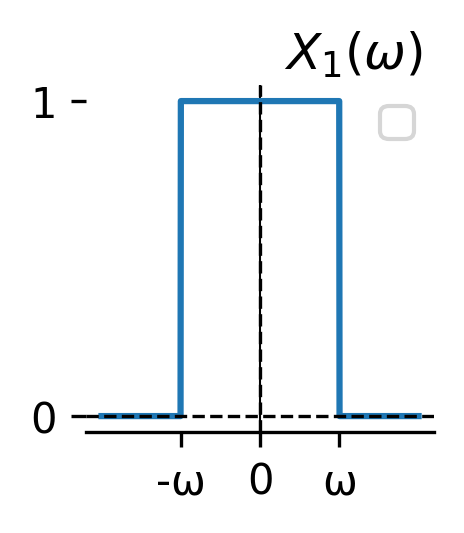
\includegraphics[width=0.4\columnwidth, height=2.5cm]{2023/EC/49/figs/plot.png}\hfill
    \begin{tabular}{c}
        {\sffamily\raisebox{1.75cm}{*}} 
    \end{tabular}\hfill
    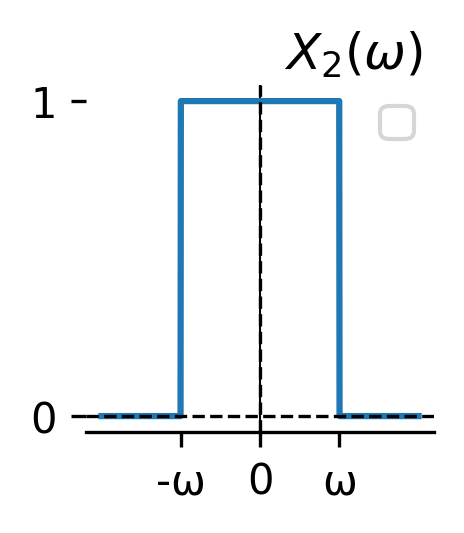
\includegraphics[width=0.4\columnwidth, height=2.5cm]{2023/EC/49/figs/plot4.png}
    
    \caption{}
    \label{fig:overall}
\end{figure}

\begin{align}
\left(\frac{\sin(\omega t)}{\pi t}\right)^2  \xleftrightarrow{\mathcal{F}} X_3(\omega) 
\end{align}
\begin{figure}[h!]
    \centering
    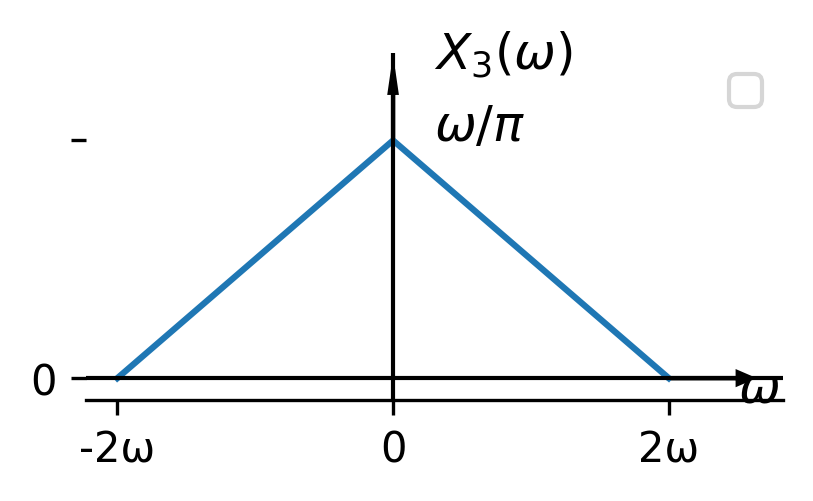
\includegraphics[width=0.5\columnwidth, height=3cm]{2023/EC/49/figs/plot1.png}
    \caption{}
    \label{fig:sr11}
\end{figure}
\begin{align}
\pi\left(\frac{\sin(\omega t)}{\pi t}\right)^2 \xleftrightarrow{\mathcal{F}} X_4(\omega)
\end{align}
\begin{figure}[h!]
    \centering
    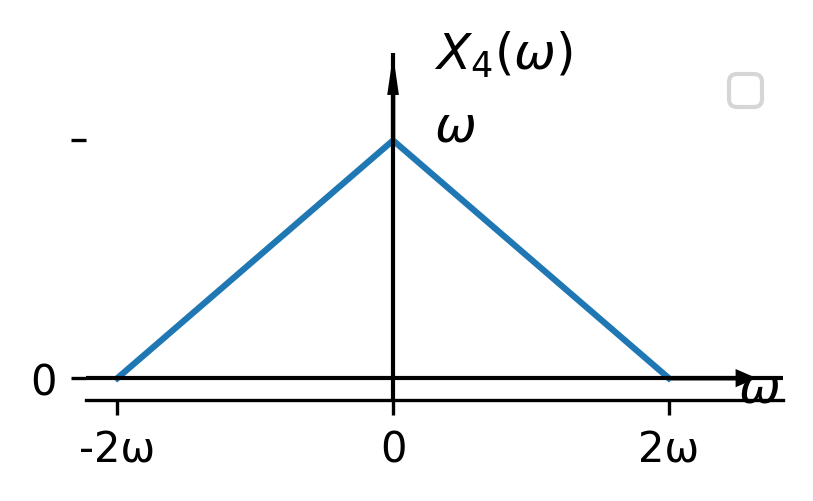
\includegraphics[width=0.5\columnwidth, height=3cm]{2023/EC/49/figs/plot2.png}
    \caption{}
    \label{fig:sr12}
\end{figure}
    \begin{align}
\text{From modulating property:} \nonumber \\
        f(t) \cos(\omega_0 t) \xleftrightarrow{\mathcal{F}} \frac{1}{2} \left[F(\omega + \omega_0) + F(\omega - \omega_0)\right]
    \end{align}

    \begin{align}
        H(\omega) &= \frac{1}{2} \left[F(\omega + 10\omega) + F(\omega - 10\omega)\right]
    \end{align}

\begin{figure}[h!]
    \centering
    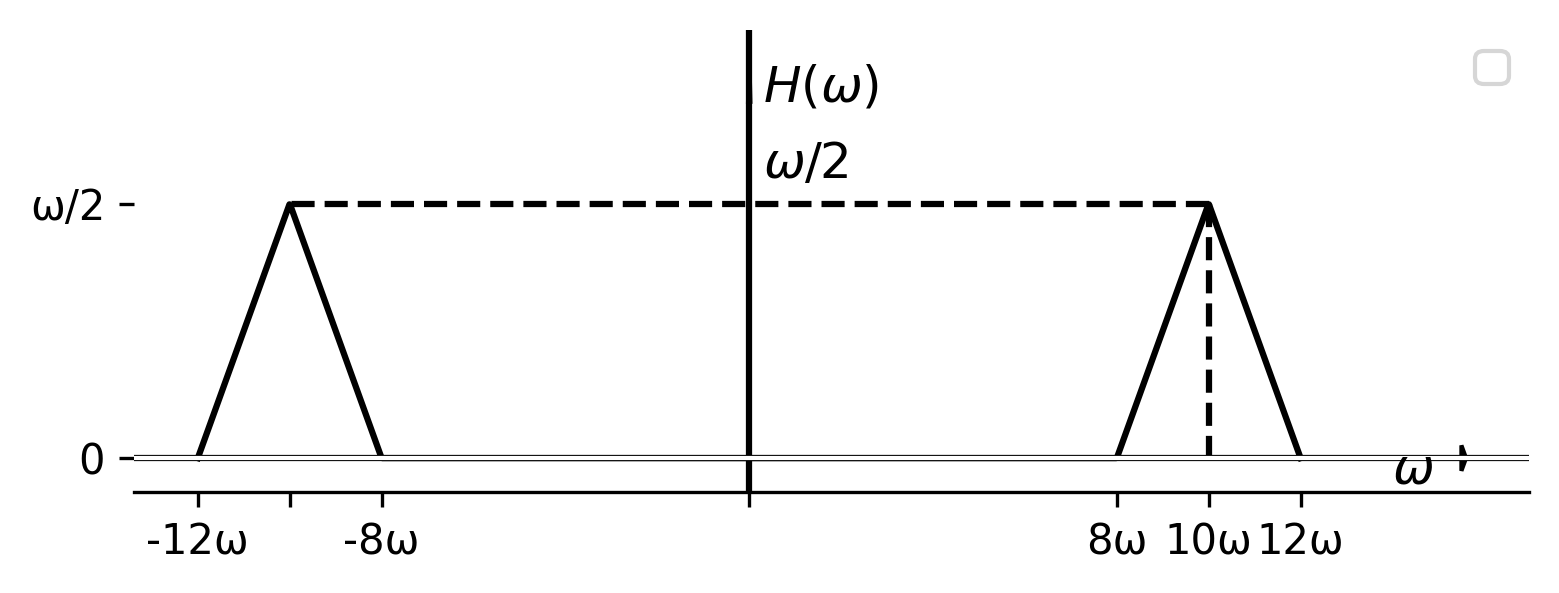
\includegraphics[width=0.7\columnwidth,height=2.5cm]{2023/EC/49/figs/plot3.png}
    \caption{}
    \label{fig:sr13}
\end{figure}
\begin{equation}
    \frac{\frac{\omega}{2} - 0}{10\omega - 12\omega} = \frac{|H(10.5\omega)| - 0}{10.5\omega - 12\omega}
\end{equation}

\begin{align}
A = |H(10.5\omega)| &= \frac{3}{8}\omega \quad \text{and} \quad  \theta= \angle H(10.5\omega) = 0^\circ
\end{align}

The output \(y(t)\):
\begin{align}
y(t) &= \frac{3}{8}\omega \cdot 10 \cos(10.5 \omega t) \\
&= \frac{15}{4}\omega \cos(10.5 \omega t)
\end{align}
\begin{figure}[h!]
    \centering
    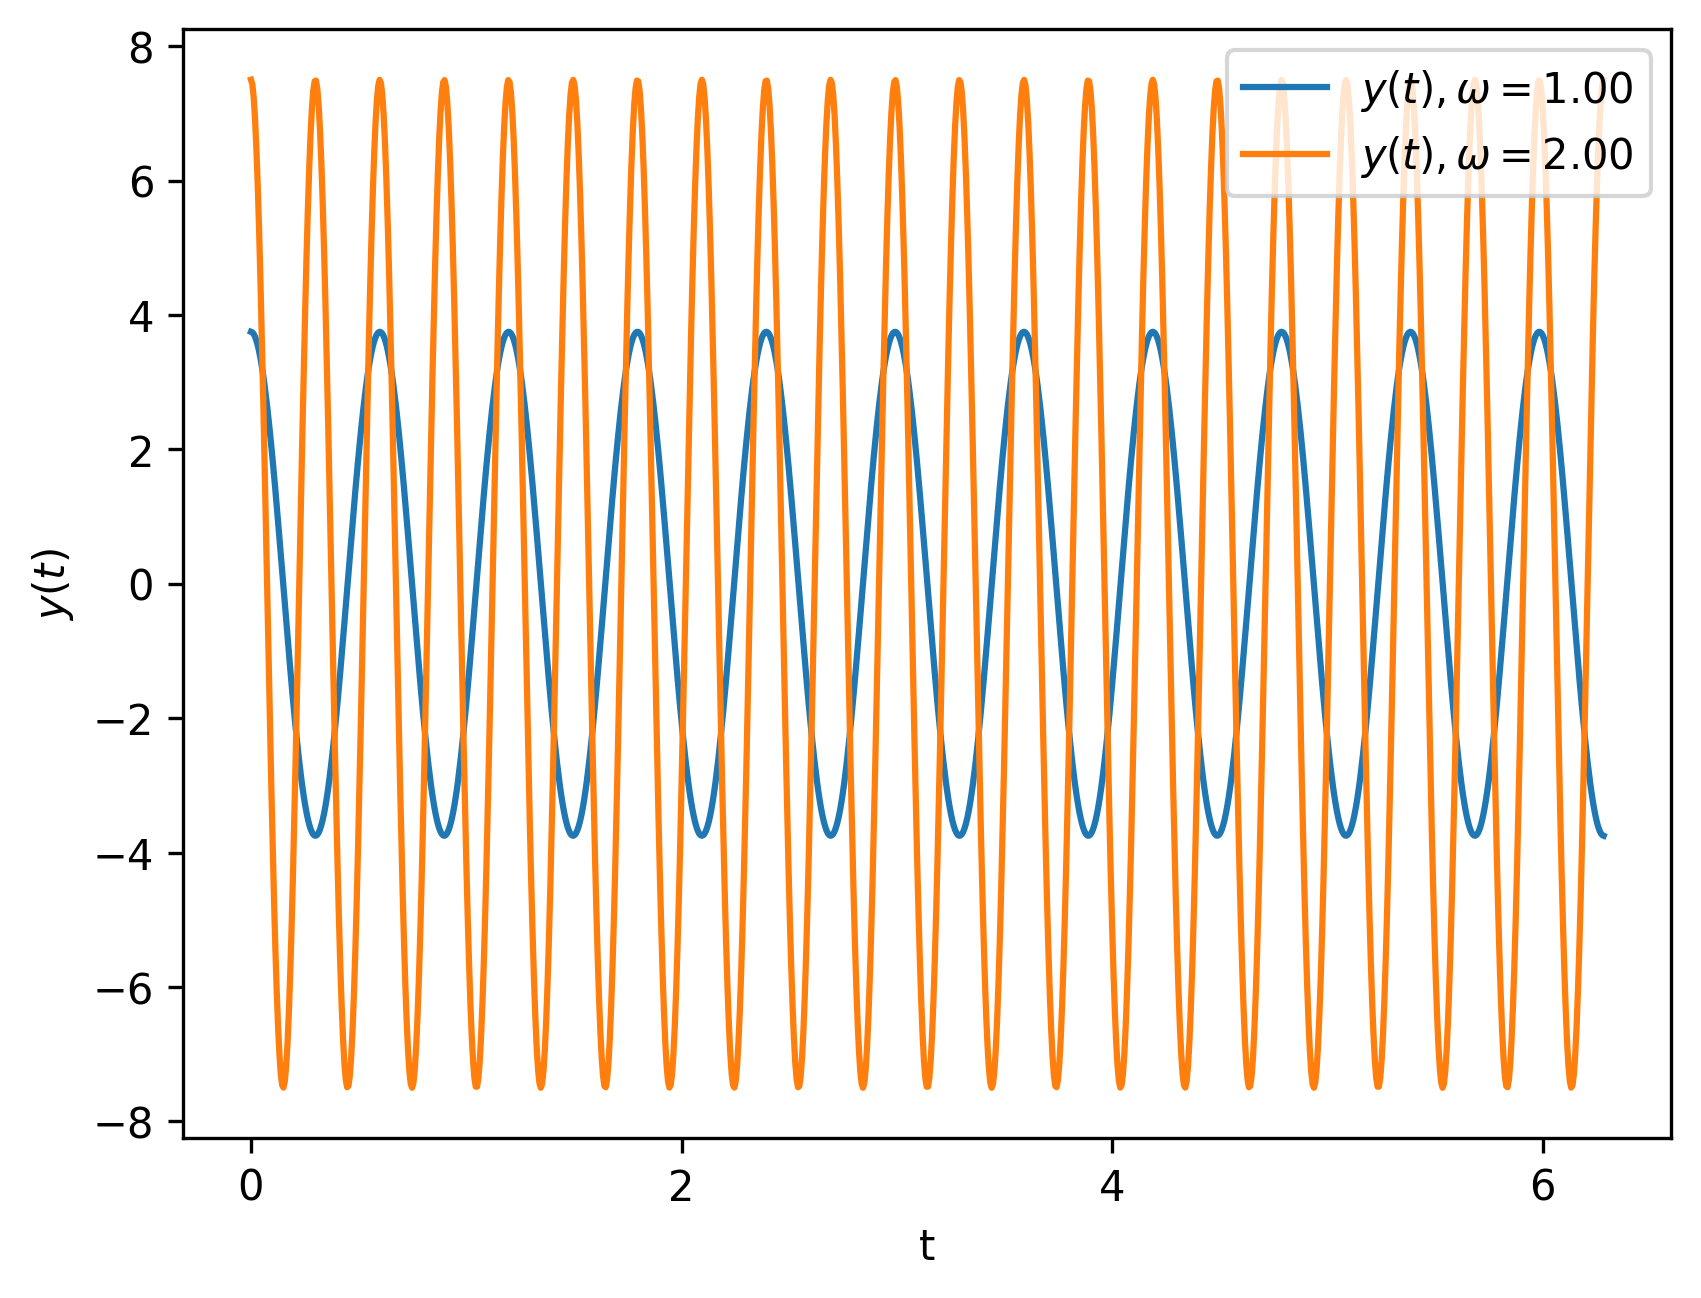
\includegraphics[width=\columnwidth]{2023/EC/49/figs/plot5.png}
    \caption{}
    \label{fig:sr14}
\end{figure}
%\end{document}

